%# -*- coding: utf-8 -*-
% !TeX encoding = UTF-8 Unicode
% !TeX spellcheck = en_US
% !TeX TS-program = xelatex
%~ \XeTeXinputencoding "UTF-8"
% vim:ts=4:sw=4
%
% 以上设定默认使用 XeLaTex 编译,并指定 Unicode 编码,供 TeXShop 自动识别

\chapter{app-wpapw}

\section{High Level Design}



\begin{enumerate}
  \item 使用 flowchart 将处理流程初步理清
  \item 使用 \href{http://www.cascading.org/}{Cascading}/MapReduce 实现系统
  \item 测试
\end{enumerate}


\subsection{介绍}


REF:
\href{https://suprafortix.wordpress.com/tag/rockyou-txt/}{Hashcat Password Cracking, such as no rule and rule crack}
\href{https://hashcat.net/wiki/doku.php?id=cracking_wpawpa2}{hashcat wiki, dic+bruteforce+rule}


\begin{lstlisting}[language=bash]
# command line to crack with dictionary
hashcat -m 2500 for-science-hs.hccap ZD_Tirom_Merger+Trim_8-16_v09d.txt

# with rule
hashcat -m 2500 -r rules/best64.rule for-science-hs.hccap ZD_Tirom_Merger+Trim_8-16_v09d.txt
\end{lstlisting}



\begin{enumerate}
  \item input task:
  convert the input to various actions:
 1. dictionary
 2. brute force (pattern) + rules
 detect how many GPU cards, "hashcat -I"
 use a global variable to store the used card(or left card?)

 for example, ATTXXX, will be consider to run both dic and brute force,
 and brute force is base on the default factory password, which is 10 digital numbers.
 so the software will generate following internal lines:

\begin{lstlisting}[language=bash]
#  <type>, <filename>, <pw type>,   <pw dictionary>
   wpa, test.hs.hccap, dictionary, wordlist1.txt,
   wpa, test.hs.hccap, dictionary, wordlist2.txt,
   wpa, test.hs.hccap, dictionary, wordlist3.txt,
   wpa, test.hs.hccap, dictionary, wordlist4.txt,
   wpa, test.hs.hccap, dictionary, wordlist5.txt,
   wpa, test.hs.hccap, dictionary, wordlist6.txt,

#  <type>, <filename>, <pw type>,   <pw pattern>
   wpa, test.hs.hccap, mask, 0?d?d?d?d?d?d?d?d?d,
   wpa, test.hs.hccap, mask, 1?d?d?d?d?d?d?d?d?d,
   wpa, test.hs.hccap, mask, 2?d?d?d?d?d?d?d?d?d,
   wpa, test.hs.hccap, mask, 3?d?d?d?d?d?d?d?d?d,
   wpa, test.hs.hccap, mask, 4?d?d?d?d?d?d?d?d?d,
   wpa, test.hs.hccap, mask, 5?d?d?d?d?d?d?d?d?d,
   wpa, test.hs.hccap, mask, 6?d?d?d?d?d?d?d?d?d,
   wpa, test.hs.hccap, mask, 7?d?d?d?d?d?d?d?d?d,
   wpa, test.hs.hccap, mask, 8?d?d?d?d?d?d?d?d?d,
   wpa, test.hs.hccap, mask, 9?d?d?d?d?d?d?d?d?d,

#  <type>, <filename>, <pw type>,   <pw pattern>, <rule>
   wpa, test.hs.hccap, rule, 0?d?d?d?d?d?d?d?d?d, best64
   wpa, test.hs.hccap, rule, 1?d?d?d?d?d?d?d?d?d, best64
   wpa, test.hs.hccap, rule, 2?d?d?d?d?d?d?d?d?d, best64
   wpa, test.hs.hccap, rule, 3?d?d?d?d?d?d?d?d?d, best64
   wpa, test.hs.hccap, rule, 4?d?d?d?d?d?d?d?d?d, best64
   wpa, test.hs.hccap, rule, 5?d?d?d?d?d?d?d?d?d, best64
   wpa, test.hs.hccap, rule, 6?d?d?d?d?d?d?d?d?d, best64
   wpa, test.hs.hccap, rule, 7?d?d?d?d?d?d?d?d?d, best64
   wpa, test.hs.hccap, rule, 8?d?d?d?d?d?d?d?d?d, best64
   wpa, test.hs.hccap, rule, 9?d?d?d?d?d?d?d?d?d, best64
\end{lstlisting}

  \item the hashcat will run according to the lines generated,
and output lines if the password found:
\begin{lstlisting}[language=bash]
#  <type>, <filename>, <result>,   <password>
   wpa, test.hs.hccap, found, 1234567890
   wpa, test.hs.hccap, notfound,
\end{lstlisting}

  \item the output lines are sorted and remove duplicated lines,
if there's success line, then remove other failed lines of the same config.

\end{enumerate}


dictionary
? support compressed?
kali default /usr/share/wordlists/
such as rockyou.txt




the gpu card run the hash code in speed of around 50k,
specifically, it is 77366 H/s for a Tesla K40m,
60960 H/s for a NVIDIA GeForce GTX 960M,
and 28989 H/s for a NVIDIA GeForce GTX 745.
\url{http://crackingservice.com/?q=benchmark}

we split the pattern to multiple segments,
and also split the dictionary to multiple segments,
so each segment contains same number of words;

the average time for switching tasks would be 2 seconds,
and we want this time is less than 1% of the total time,
so the we want a word/pattern segment involved in computing at least 2/1% =200 seconds,

so the number of word for each segment is 60k * 200 = 12000k
we select 10m as the number of word in the segmen



\subsection{整体结构}
图 \ref{fig:system} 是整个系统的运行框架。

\definecolor{vidtransoriginfile}{HTML}{D7FE39}
\definecolor{vidtranstmpfile}{HTML}{EDE80F}
\definecolor{vidtransfinalfile}{HTML}{FFE985}
\definecolor{vidtransprocess}{HTML}{FEA93E}
\definecolor{vidtransfuncio}{HTML}{DADAFF}
\begin{figure}\centering
  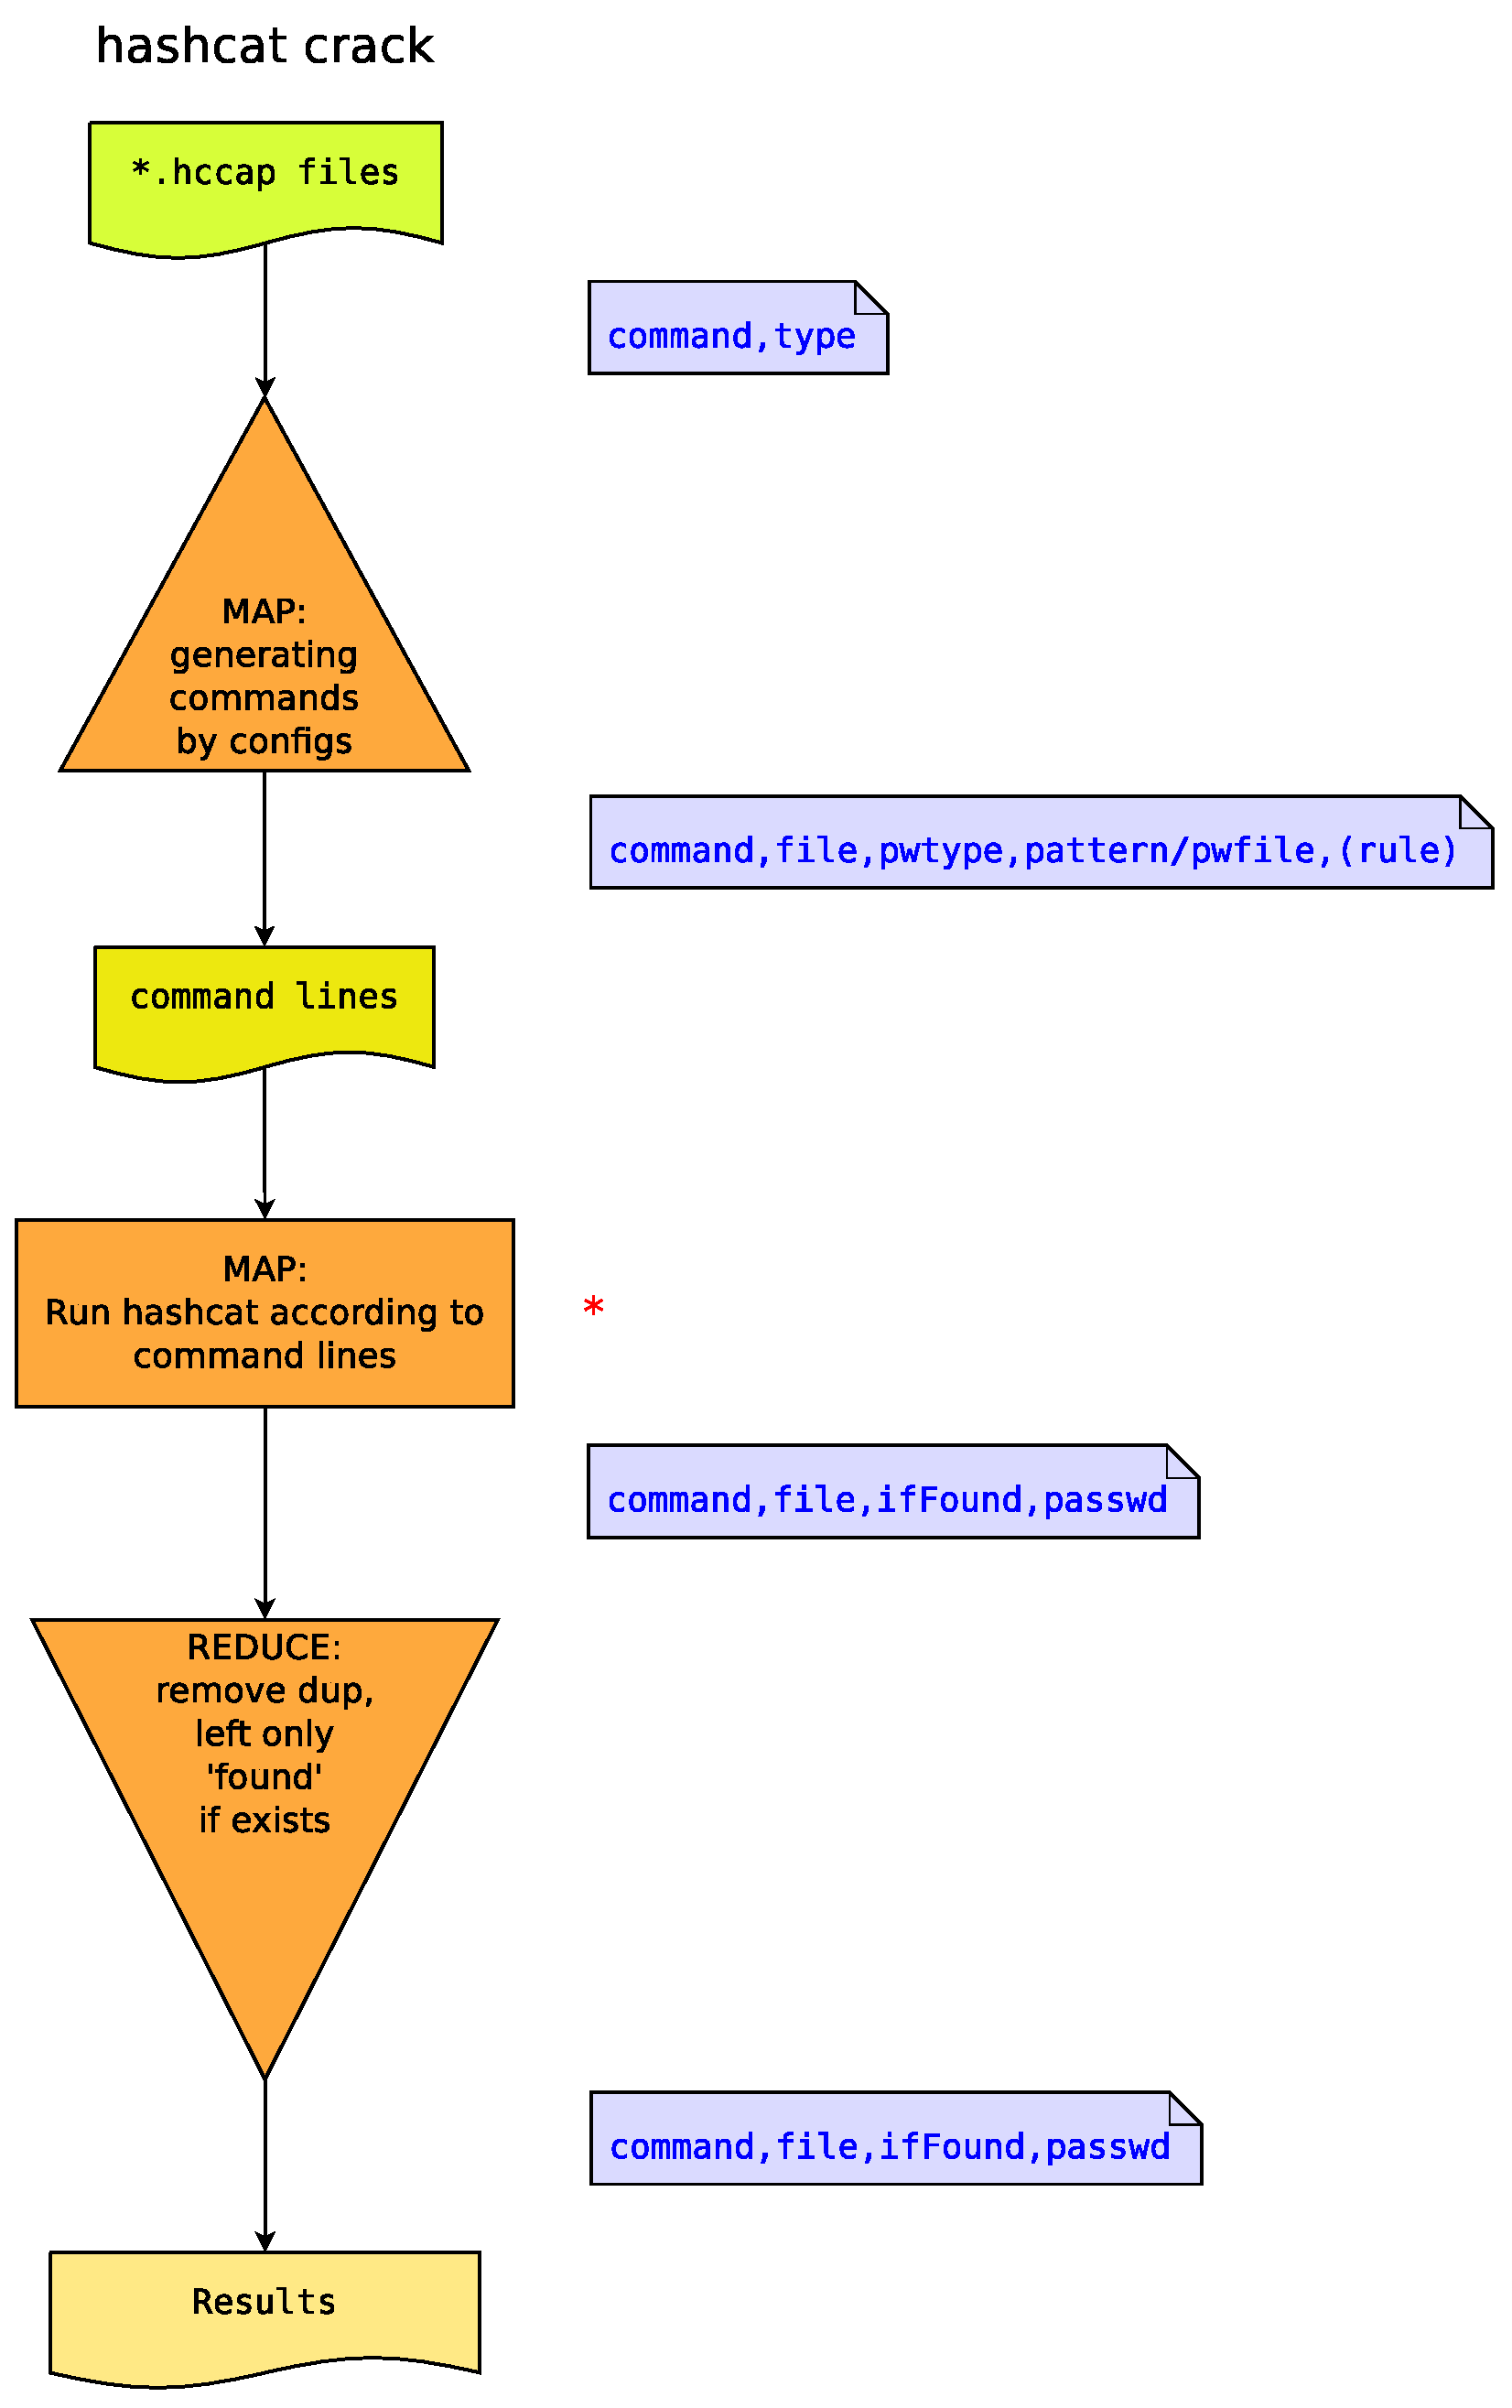
\includegraphics[width=0.5\textwidth]{flowchart-mr-wpapw}
  \caption{The system.
    The text in \fcolorbox{black}{vidtransoriginfile}{this color} is the original input file.
    The text in \fcolorbox{black}{vidtranstmpfile}{this color} is the temp file.
    The text in \fcolorbox{black}{vidtransfinalfile}{this color} is the final output file.
    The text in \fcolorbox{black}{vidtransprocess}{this color} is process block.
    The text in \fcolorbox{black}{vidtransfuncio}{\textcolor[HTML]{0000FF}{this color}} is the input/output of one process block.
The process blocks signed by a \textcolor[HTML]{FF0000}{*} are the blocks cost most of the processing time.
  }\label{fig:system}
\end{figure}



\section{Low Level Design}
TODO


\section{Performance}
TODO
